\section{Results}
\label{sec:results}

We evaluate the performance of \gptlarge and \gptmini on \benchmark. Our primary analysis examines the models' performance across the trigger and action types.
\para{Main Results: Trigger Type.}
Both models show a significant performance drop as the trigger becomes more abstract. As shown in \Tabref{tab:trigger_results}, \gptlarge achieves a 66.0\% adherence score on lexical triggers, which drops to 52.0\% for conceptual and 38.0\% for structural triggers. This demonstrates that models excel at keyword-based monitoring but struggle to maintain structural or semantic consistency over long generations (see \figref{fig:trigger_comparison}).

\begin{figure}[t]
\centering
\begin{subfigure}[b]{0.48\textwidth}
    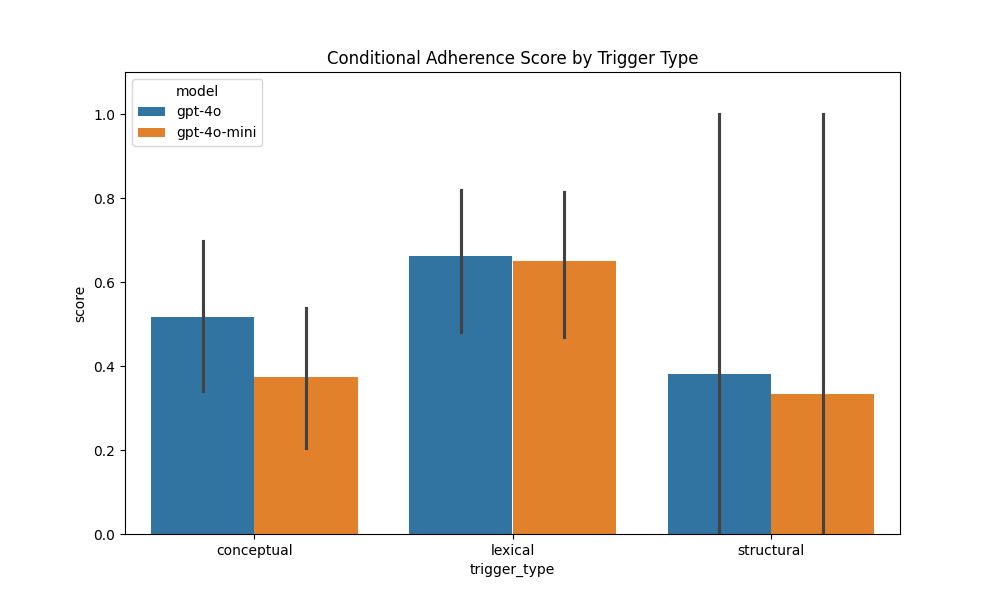
\includegraphics[width=\textwidth]{figures/trigger_comparison.png}
    \caption{Adherence by Trigger Type}
    \label{fig:trigger_comparison}
\end{subfigure}
\hfill
\begin{subfigure}[b]{0.48\textwidth}
    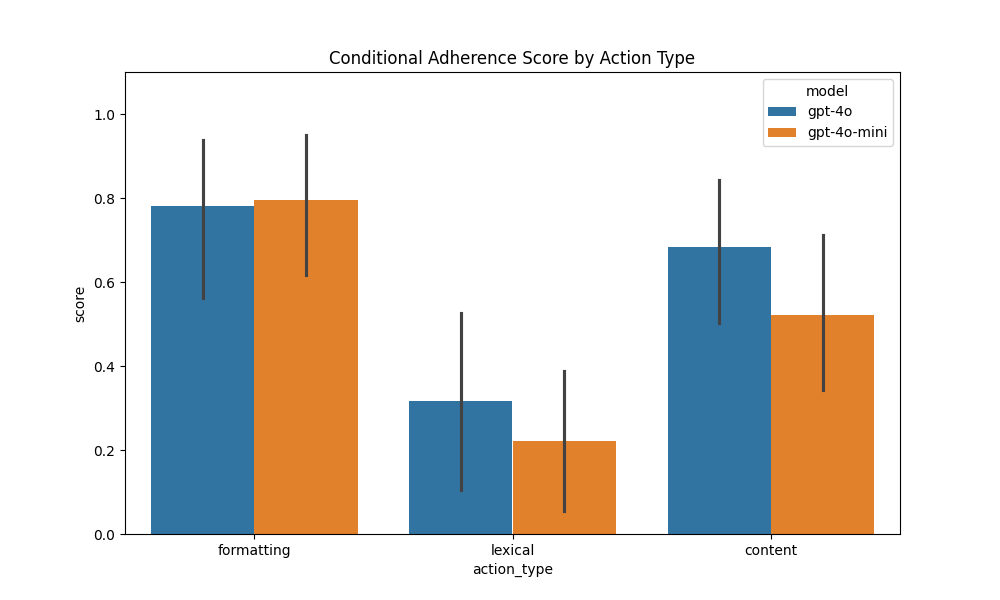
\includegraphics[width=\textwidth]{figures/action_comparison.png}
    \caption{Adherence by Action Type}
    \label{fig:action_comparison}
\end{subfigure}
\caption{Comparison of model performance across trigger and action types. Both models show similar trends, with \gptlarge generally outperforming \gptmini on more complex tasks.}
\label{fig:main_comparison}
\end{figure}

\begin{table}[h]
\centering
...
\caption{Adherence Scores by Trigger Type for \gptlarge and \gptmini. Models show a significant drop in performance for conceptual and structural triggers.}
\begin{tabular}{@{}lccc@{}}
\toprule
\textbf{Model} & \lexical & \conceptual & \structural \\ \midrule
\gptlarge & {\bf 0.66} & {\bf 0.52} & {\bf 0.38} \\
\gptmini & 0.65 & 0.37 & 0.33 \\ \bottomrule
\end{tabular}
\label{tab:trigger_results}
\end{table}

\para{Main Results: Action Type.}
Interestingly, models perform better at formatting and content actions than at lexical insertions (\Tabref{tab:action_results}). While \gptlarge achieves a high 78.0\% adherence score for formatting actions, its performance for lexical actions is remarkably low (32.0\%). This suggests that while models can easily apply a global style, they find it difficult to insert specific keywords in a way that remains coherent with the generated text.

\begin{table}[h]
\centering
\caption{Adherence Scores by Action Type. Models excel at formatting and content actions but struggle with lexical insertions.}
\begin{tabular}{@{}lccc@{}}
\toprule
\textbf{Model} & \lexical & \formatting & \content \\ \midrule
\gptlarge & {\bf 0.32} & {\bf 0.78} & {\bf 0.68} \\
\gptmini & 0.22 & 0.79 & 0.52 \\ \bottomrule
\end{tabular}
\label{tab:action_results}
\end{table}

\para{Scalability of Conditional Capacity.}
The difference between \gptlarge and \gptmini is most pronounced in conceptual triggers (+40\% improvement for \gptlarge) and content actions (+30\% improvement). This suggests that ``large'' models have a more robust internal representation of abstract concepts and are better at generating content that satisfies complex conditions. However, both models perform poorly on structural triggers, indicating that structural awareness remains a challenge even for state-of-the-art models.

\para{False Positive Analysis.}
Our results show a high rate of false positives across both models. On average, \gptlarge exhibited ~0.8 lexical false positives per rule. This indicates that models often ``leak'' conditional actions into parts of the generation where the trigger was never present. For example, a rule to bold sentences that mention a specific word might result in several unrelated sentences being bolded as well. This suggests that the conditional instruction acts more like a global bias than a precise logical trigger.

{\bf What is the cause of this bias?} We hypothesize that once a model is primed with a conditional rule, it maintains a high degree of activation for that rule, which leads to over-application. This is consistent with previous findings on semantic bias and content effects in LLM reasoning \cite{dasgupta2022content}.
